\section{Pointers: Important Concepts}
\label{sec:Pointers-ImportantConcepts}
%~\cref{sec:Pointers-ImportantConcepts}
\subsection{Passing Arguments with Pointers}
\label{subsec:Pointers-02-ImportantConcepts-PassingArguments}
%~\cref{subsec:Pointers-02-ImportantConcepts-PassingArguments}

There are three forms of passing arguments to a function. One of them is possible through the use of pointers.
\begin{itemize}
    \item Passing by value
    \item Passing by reference with a reference argument\\
    \begin{minipage}{\MPWxXXSxLISTING\textwidth} % = 0.36 times \textwidth
    \vspaceTextToListing % =\vspace{0.1cm}
    \begin{CPPCode}
int x{2};
SquareByReference(x)
cout ¿<¿¿<¿ "x is" ¿<¿¿<¿ x 
    \end{CPPCode}
    \begin{Terminal}
Output:
x is 4
    \end{Terminal}
    \end{minipage}
    \hspaceListingXSToListingXS
    \begin{minipage}{\MPWxXSxLISTING\textwidth} % = 0.36 times \textwidth
    \vspaceTextToListing % =\vspace{0.1cm}
    \begin{CPPCode}
squareByReference(int&) // Prototype

squareByReference(int& numberRef)
{
    numberRef *= numberRef;
}
    \end{CPPCode}
    \end{minipage}
    
    \item Passing by reference with a pointer argument\\
    \begin{minipage}{\MPWxXXSxLISTING\textwidth} % = 0.36 times \textwidth
    \vspaceTextToListing % =\vspace{0.1cm}
    \begin{CPPCode}
int x{2};
SquareByPtrRef(&x)
cout ¿<¿¿<¿ "x is" ¿<¿¿<¿ x 
    \end{CPPCode}
    \begin{Terminal}
Output:
x is 4
    \end{Terminal}
    \end{minipage}
    \hspaceListingXSToListingXS
    \begin{minipage}{\MPWxXSxLISTING\textwidth} % = 0.36 times \textwidth
    \vspaceTextToListing % =\vspace{0.1cm}
    \begin{CPPCode}
squareByPtrRef(int*)// Prototype

squareByPtrRef(int* nPtr)
{
    *nPtr = *nPtr * *nPtr
}
    \end{CPPCode}
    \end{minipage}
\end{itemize}

\noindent Passing a variable by reference with a pointer \textbf{does not actually pass anything by reference} a pointer to that variable is passed by value and is copied into the function’s corresponding pointer parameter. The called function can then access that variable in the caller simply by \textbf{dereferencing} the pointer, thus accomplishing pass-by-reference.

\subsection{\CppCommonCode{const} with Pointers}
\label{subsec:Pointers-02-ImportantConcepts-02-const-with-Pointers}
%~\cref{subsec:Pointers-02-ImportantConcepts-02-const-with-Pointers}
Keyword \CppCommonCode{const} enables you to inform the compiler that the value of a particular variable should \textbf{not} be modified. This is usefull when using built-in arrays (See Section~\cref{subsec:Built-In-Arrays}) as they are passed by reference and could easily be changed in the called funcion. An attempt to modify a const value is a compilation error.







%%%%%%%%%%%%%%%%%%%%%%%% END going through array
% no numbers listing
% \begin{lstlisting}[frame=tlrb,numbers=none,mathescape=true,escapechar=\%,columns=flexible]

% \begin{minipage}{.9\textwidth}
% \begin{lstlisting}[frame=tlrb,showlines=htrue,firstnumber=1,mathescape=true,escapechar=\%,columns=flexible]
% //code here
% \end{lstlisting}
% \end{minipage}

% \begin{lstlisting}[frame=tlrb,showlines=htrue,firstnumber=1,mathescape=true,escapechar=\%,columns=flexible]
% //Program 12.1
% \end{lstlisting}
    
%reference:
%~\ref{tab:t_ch11_UART_Registers} tab:t_ch12_edgeTriggeredModes
%~\ref{fig:RT_ch01} 
%\texttt{Ascii}
%\texttt{UART}
%\texttt{mailbox}
%\texttt{FIFO}
%\texttt{I/O}
%\underline{}
%$\texttt{b}_0$
%\sim = ~

%percent
%n%\%%10;

%for loops
% \newcounter{nnCount}
% \forloop{nnCount}{0}{\value{nnCount}<8}{&IME }  
% \forloop{nnCount}{0}{\value{nnCount}<8}{&PMC\arabic{nnCount} }

%Apostroph:
%\textquotesingle

%Equation array
% \begin{eqnarray*}
%  & = & \text{minimun}\\
%  & = & \text{maximun}\\
%  & = &  \\
%  & = & \\
%  & = & 
% \end{eqnarray*}

% \begin{description}
% \item[Remark 1] If
% \end{description}

% \begin{description}
% \item[Remark 1] If
% \item[Remark 2] An
% \item[Remark 3] With 
% \end{description}

%Poner figura
% \begin{figure}[!h] %%%%%%%%%%%%%%%%%%%%%%% Begin Figure Directory
% \centering
% \includegraphics[width=0.70\linewidth]{figuresRT/ch06/RT-CH06-
% \caption{Free-space management.}
% \label{fig:ch01_00}
% %~\ref{ffig:ch01_00} 
% \end{figure}       %%%%%%%%%%%%%%%%%%%%%%% End Figure

%Poner Figura con minipages
% %begin minipages
% \begin{minipage}{.45\textwidth}
% %here some text.
% \end{minipage}
% \begin{minipage}{.55\textwidth}
% %and here the image.
% \centering
% \includegraphics[width=0.95\linewidth]{figures/ch12/ch12_lab12_squeme1.pdf}
% \captionof{figure}{Lab 12 diagram connections}
%\label{fig:RT_ch04_MACQ-EXAMPLE-01-oldDataIsLost}
%~\ref{fig:RT_ch04_MACQ-EXAMPLE-01-oldDataIsLost} 
% \end{minipage}
% \vspace{0.5cm}
% %end minipages

% %Poner Figura y al costado codigo
% %begin minipages
% \begin{minipage}{.60\textwidth}
% %%%%%%%%%%%%%%%%%%%%%%%%%%%%%%%%%Figure Selection Statement - while
% \centering
% 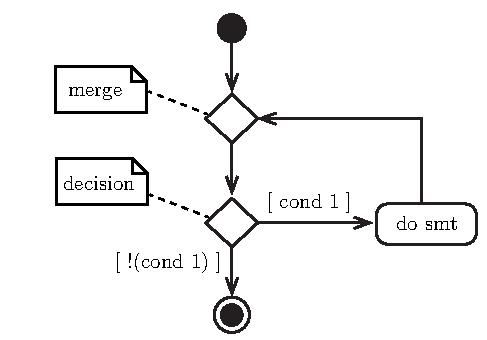
\includegraphics[width=0.50\linewidth]{01_Basics/figures/uml/IterationStatement-00-UML-while.pdf}
% \captionof{figure}{UML \texttt{while} Activity Diagram Representation}
% \label{fig:ch01_Basics_UML_IterationStatement-00-while}
% %~\ref{fig:ch01_Basics_UML_IterationStatement-00-while} 
% %%%%%%%%%%%%%%%%%%%%%%%%%%End figure
% \end{minipage}
% \begin{minipage}{.25\textwidth}
% %%%%%%%%%%%%%%%%%%%%%%%%%%%%%%%%%Begin code
% \begin{lstlisting}[frame=tlrb,numbers=none,mathescape=true,escapechar=\%,columns=flexible]
% some awesome code here
% \end{lstlisting}
% %%%%%%%%%%%%%%%%%%End Code
% \end{minipage}
% \vspace{0.5cm}
% %end minipages


%\begin{enumerate}
%	\item Initialize timer and directions registers
%    \item Specify initial state
%    \item Perform FSM controller
%   \begin{enumerate}
%    	\item Call an output function, which depends on the state
%        \item Delay, which depends on the state
%        \item Call an input function to get the status of the coin sensors
%        \item Change states, which dependes on the state and the input
%    \end{enumerate}
%\end{enumerate}

% \begin{enumerate}
% 	\item Current instruction is finished,
%     \item Eight registers are pushed on the stack,
%     \item LR is set to 0xFFFFFFF9,
%     \item IPSR is set to the interrupt number,
%     \item PC is loaded with the interrupt vector
% \end{enumerate}

% Itemize categoriza poniendo (.) en lugar de números
% \begin{itemize} 
% 	\item I
% 	\item I
% 	\item Y
% 	\item Y
% 	\item Y
% 	\item Y
% 	\item 
% \end{itemize}

% \begin{table}[!h]
% \centering
% \begin{tabular}{|l|l|l|} \hline
% $p$ & bit Field & Interrupt         \\\hline
% $3$ & \bitsRange[31]{29} & Interrupt [$4m+3$]  \\\hline
% $2$ & \bitsRange[23]{21} & Interrupt [$4m+2$]  \\\hline
% $1$ & \bitsRange[15]{13} & Interrupt [$4m+1$]  \\\hline
% $0$ & \bitsRange[7]{5} & Interrupt [$4m$]   \\\hline
% \end{tabular}
% \caption{pasteCaption}
% \label{tab:t_rt_ch04_}
% ~\ref{tab:t_rt_ch04_}
% \end{table}

% Insertar URL
%\url{https://www.osha.gov/Publications/laboratory/OSHAfactsheet-laboratory-safety-noise.pdf}\\

% \newcommand{\bitsRange}[2][50]{\texttt{{#1}-{#2}}}
% \newcommand{\CustomHex}[2][0000]{\texttt{0x{#1}.{#2}}}
% \newcommand{\GPIOPort}[1]{\texttt{GPIO\_PORT{#1}}}
% \newcommand{\GPIOPortR}[2][A]{\texttt{GPIO\_PORT{#1}\_{#2}\_R}}
% \newcommand{\GPIOPortHandler}[1]{\texttt{GPIO\_PORT{#1}\_Handler}}
% \newcommand{\HandlerISR}[1]{\texttt{#1\_Handler}}
% \newcommand{\IRQnr}[1]{\texttt{{#1}}}
% \newcommand{\NVICPRI}[1]{\texttt{NVIC\_PRI{#1}\_R}}
% \newcommand{\NVICEN}[1]{\texttt{NVIC\_EN{#1}\_R}}
% \newcommand{\NVICDIS}[1]{\texttt{NVIC\_DIS{#1}\_R}}
% \newcommand{\Ttimer}[2][A]{\texttt{Timer\_{#2}{#1}}}
% \newcommand{\xNrbit}[1]{$#1$-\texttt{bit}}
% \newcommand{\xNrbits}[1]{$#1$-\texttt{bits}}
% \newcommand{\camouflagegreenCellColor}{\cellcolor[rgb]{0.47, 0.53, 0.42}}
% \newcommand{\lavenderCellColor}{\cellcolor[rgb]{0.9, 0.9, 0.98}}
% \newcommand{\volties}[2][0]{$\si{{#1}\volt}_{#2}$}
% \newcommand{\volti}[1]{$\si{{#1}\volt}$}
% \newcommand{\voltiposi}[1]{$+\si{{#1}\volt}$}
% \newcommand{\voltinega}[1]{$-\si{{#1}\volt}$}